% GENERATED FROM typst/manual/sections/05_solar_system_field_tests.typ BY scripts/typ2tex.py (v1.0.0) — DO NOT EDIT.
% Edit canonical Typst under typst/ and regenerate with: python3 scripts/typ2tex.py --root . --outdir latex

\section{Solar Observable-Map Fixtures}\label{manual:solar-system-field-tests}

\paragraph{Calculation card.}
The Sun/body/window declarations and carried O0 values below supply exact
rational residual arithmetic---verified by vector \texttt{RC-040}
(\texttt{dec\_solar\_o0\_boundary\_audit}, \texttt{solar\_o0\_boundary\_dec\_audit.csv})
under the explicit gate \texttt{HOLD\_MISSING\_NATIVE\_SOLAR\_PRODUCER}---and do not
constitute a replayed native solar evaluator. The $42.98$ perihelion and $1.75$
bending references are theory benchmarks. The redshift record separately
identifies a reference prediction and a measured estimate with uncertainty.
This application must supply its native construction, observable map, source
certificates, and uncertainty before physical prediction; see
\secref{manual:calculation-spine}.

\aodnoteblock{Scope}{This section carries solar-system observable-map comparison fixtures. Each record declares its solar-system scope, names the observable map, carries a comparison value, attaches an external reference target, and records residual, percent error, source citation, and audit.}

\aodnoteblock{Data-support class}{Solar records are O0 observable-map fixtures. Each row records map value, target, residual/error, and citation inside the declared observable-map support class.}

\subsection{Shared solar-system declaration}\label{manual:solar:shared}

Declare a solar field scope

\[
\mathbf{a}_{\odot}\vdash(F_{\odot},R_{\odot},\partial R_{\odot},\omega_{\odot}),\qquad B_{\odot}=(\partial F_{\odot},\omega_{\odot}).
\]

For a body, signal, or transfer record $x$, declare a comparison boundary/window

\[
B_x=(\partial F_x,\omega_x).
\]

Each record carries a frozen O0 map-value comparison and its external reference target.

\begin{figure}[H]
\centering
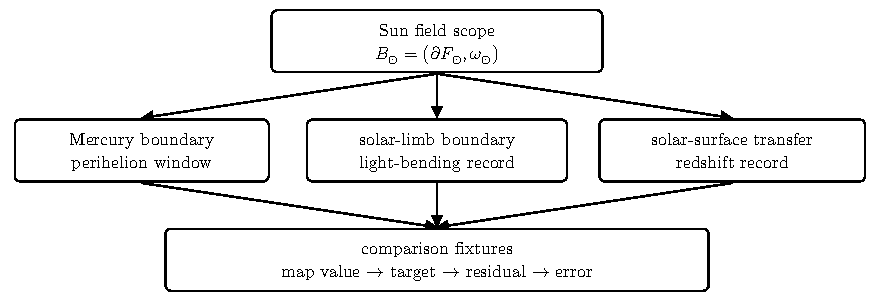
\includegraphics[width=\linewidth]{figures/generated/solar-system-spine.pdf}
\caption{Solar-system observable-map comparison spine. The records carry map values, targets, residuals, percent errors, and source citations.}
\label{fig:manual-solar-system-spine}
\end{figure}

\[
\boxed{\text{Solar-system records carry O0 observable-map comparisons.}}
\]

\subsection{SADAR observable bridge}\label{manual:solar:observable-export-bridge}

Native solar-system evaluation requires a Sun-field cycle family evaluated by $\SADARop_B$ and a declared observable comparison map with signature

\[
\mathcal{O}_{x,\AO}=\mathcal{G}_x[RCD,\rho^D,\rho^D_{\omega},p^D,\varphi,\mathbf{A}_F,J^D_{\partial R};B_x].
\]

The three observable-map comparison fixtures record the following map signatures:

\[
\Delta\varpi_{\mathrm{Hg},\AO}=\mathcal{G}_{\mathrm{peri}}[\mathbf{A}_{F_{\odot}}(B_{\mathrm{Hg}}),J^D_{\partial R}(\omega_{\mathrm{cy}};B_{\mathrm{Hg}})],
\]

\[
\delta_{\odot,\AO}=\mathcal{G}_{\mathrm{bend}}[\mathbf{A}_{F_{\odot}}(B_{\mathrm{bend}}),J^D_{\partial R}(\omega_{\mathrm{bend}};B_{\mathrm{bend}})],
\]

\[
z_{\odot,\AO}=\mathcal{G}_{\mathrm{red}}[\mathbf{A}_{F_{\odot}}(B_{\mathrm{red}}),J^D_{\partial R}(\omega_{\mathrm{red}};B_{\mathrm{red}})].
\]

The rows below carry O0 comparison values and residual arithmetic. Map definitions and evaluated native $\SADARop_B$ input certificates are not supplied for these records.
The Mercury physical-prediction gate therefore remains unevaluated. Its
future native derivation must not take the general-relativistic benchmark
as a premise; a measured comparison also needs its estimator, source locator,
reduction assumptions and uncertainty.

\subsection{Observable-map comparison table}\label{manual:solar:observable-map-table}

\begin{table}[H]
\centering
\caption{Solar-system observable-map comparison records (carried O0 values).}
\label{tab:manual-solar-observable-map-results}
{\footnotesize
\begin{tabular}{lrrrr}
\toprule
Record & A$\Omega$ value & Target & Residual & Abs. percent error \\
\midrule
Mercury perihelion & $42.9799$ arcsec/cy & $42.98$ arcsec/cy & $-0.0001$ arcsec/cy & $0.0002327\%$ \\
Solar light bending & $1.75001$ arcsec & $1.75$ arcsec & $0.00001$ arcsec & $0.0005714\%$ \\
Solar redshift & $2.11996\times10^{-6}$ & $2.12\times10^{-6}$ & $-4.0\times10^{-11}$ & $0.001887\%$ \\
\bottomrule
\end{tabular}
}
\end{table}

\begin{figure}[H]
\centering
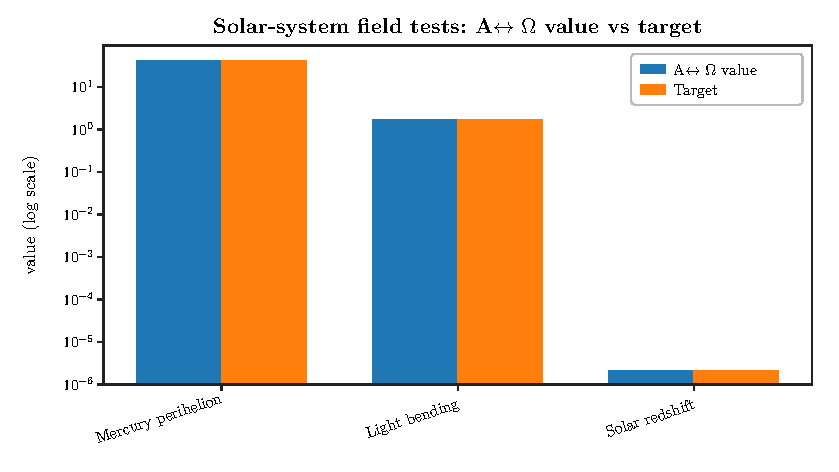
\includegraphics[width=0.92\linewidth,height=0.78\textheight,keepaspectratio]{figures/generated/solar-calculated-vs-target.pdf}
\caption{Solar-system carried observable-map values versus declared targets. The vertical axis is logarithmic; each record is compared only within its own unit/scale.}
\label{fig:manual-solar-calculated-target}
\end{figure}

\begin{figure}[H]
\centering
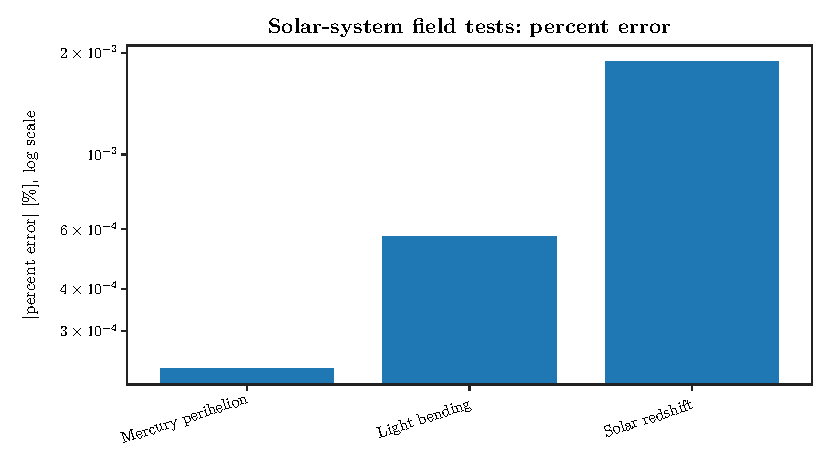
\includegraphics[width=0.92\linewidth,height=0.78\textheight,keepaspectratio]{figures/generated/solar-percent-error.pdf}
\caption{Solar-system field tests: absolute percent error.}
\label{fig:manual-solar-percent-error}
\end{figure}

\subsection{Mercury perihelion window}\label{manual:solar:mercury}

Declare

\[
\mathbf{a}_{\mathrm{Hg}}\vdash(F_{\mathrm{Hg}},R_{\mathrm{orbit}},\partial R_{\mathrm{peri}},\omega_{\mathrm{cy}}),\qquad B_{\mathrm{Hg}}=(\partial F_{\mathrm{Hg}},\omega_{\mathrm{cy}}).
\]

The observable-map value is

\[
\Delta\varpi_{\mathrm{Hg},\AO}=42.9799\,\mathrm{arcsec/century}.
\]

The theoretical reference target is

\[
\Delta\varpi_{\mathrm{Hg}}^{\mathrm{tar}}=42.98\,\mathrm{arcsec/century}.
\]

\[
\Delta_{\varpi}=-0.0001\,\mathrm{arcsec/century},\qquad|\epsilon_{\varpi}|=0.0002327\%.
\]

\aodliteraturenote{Mercury perihelion target: Will~\cite{will-mercury-2018}.}

\subsection{Solar light-bending boundary}\label{manual:solar:light-bending}

Declare

\[
\mathbf{a}_{\mathrm{bend}}\vdash(F_{\mathrm{signal}},R_{\mathrm{path}},\partial R_{\odot\mathrm{limb}},\omega_{\mathrm{bend}}),\qquad B_{\mathrm{bend}}=(\partial F_{\mathrm{signal}},\omega_{\mathrm{bend}}).
\]

The observable-map value is

\[
\delta_{\odot,\AO}=1.75001\,\mathrm{arcsec}.
\]

The theoretical reference target is

\[
\delta_{\odot}^{\mathrm{tar}}=1.75\,\mathrm{arcsec}.
\]

\[
\Delta_{\delta}=0.00001\,\mathrm{arcsec},\qquad|\epsilon_{\delta}|=0.0005714\%.
\]

\aodliteraturenote{Solar-limb light-bending target: NASA~\cite{nasa-1919-light-bending}.}

\subsection{Solar redshift transfer boundary}\label{manual:solar:redshift}

Declare

\[
\mathbf{a}_{\mathrm{red}}\vdash(F_{\mathrm{line}},R_{\mathrm{surface}},\partial R_{\mathrm{transfer}},\omega_{\mathrm{red}}),\qquad B_{\mathrm{red}}=(\partial F_{\mathrm{line}},\omega_{\mathrm{red}}).
\]

The observable-map value is

\[
z_{\odot,\AO}=2.11996\times10^{-6}.
\]

The target is

\[
z_{\odot}^{\mathrm{tar}}=2.12\times10^{-6}.
\]

\[
\Delta_z=-4.0\times10^{-11},\qquad|\epsilon_z|=0.001887\%.
\]

A separate external reference prediction is

\[
v_z^{\mathrm{tar}}=633.1\,\mathrm{m/s},
\]

with the measured comparison

\[
v_z^{\mathrm{meas}}=638\pm6\,\mathrm{m/s}.
\]

\aodliteraturenote{Solar gravitational-redshift reference prediction $633.1\,\mathrm{m/s}$ and measured comparison $638\pm6\,\mathrm{m/s}$: Heidelberg/ZAH~\cite{zah-solar-redshift}.}

\subsection{Audit hooks}\label{manual:solar:audit-hooks}

\begin{itemize}
\item Scope audit: each record declares $\mathbf{a}\vdash(F,R,\partial R,\omega)$ and $B=(\partial F,\omega)$.
\item Comparison-fixture audit: each record includes observable-map value, target, residual, percent error, and status.
\item Input audit: target values are cited in the record where they are used; residuals are computed from the declared observable-map value and declared target.
\end{itemize}

\aodprovenance{\secref{subsec:disoma-declaration};
\mainequation{main:eq:b-scoped-flux};
\mainequation{main:eq:sadar-attention-vector};
\mainequation{main:eq:window-clipped-rho};
\appref{manual:external-comparison}.}

\subsection{Five-boundary solar O0 scope separation and producer-gate ledger}\label{manual:solar:dec-o0-boundary-audit}

\paragraph{Setup and producer-gate verification (\texttt{RC-040}).}
Declare the five-boundary solar observable-map stack separating the three distinct trajectory scopes from the unsupplied native producer gate and the quarantined external target comparison:

\[
B_{\mathrm{Sun}}\to(B_{\mathrm{Hg}},B_{\mathrm{bend}},B_{\mathrm{red}})\to B_{\mathrm{gate}}\to B_{\mathrm{O0}}\to B_{\mathrm{ext}}.
\]

Vector \texttt{RC-040} (\texttt{dec\_solar\_o0\_boundary\_audit})---archived in \texttt{manual/data/boundary\_sadar/solar\_o0\_boundary\_dec\_audit.csv} and verified by \texttt{python3 -B -m manual.engine --sector boundary\_sadar} and \texttt{aod-core --verify-vectors --check-zero-float}---audits the exact rational observable-map residuals across $B_{\mathrm{Hg}}$ (closed orbital return shell), $B_{\mathrm{bend}}$ (open grazing ray chord), and $B_{\mathrm{red}}$ (radial potential climb window) while certifying \texttt{native\_sadar\_evaluated = 0} and locking every row behind \texttt{HOLD\_MISSING\_NATIVE\_SOLAR\_PRODUCER} so O0 observable-map arithmetic is never misrepresented as a native solar derivation.

\begin{figure}[H]
\centering
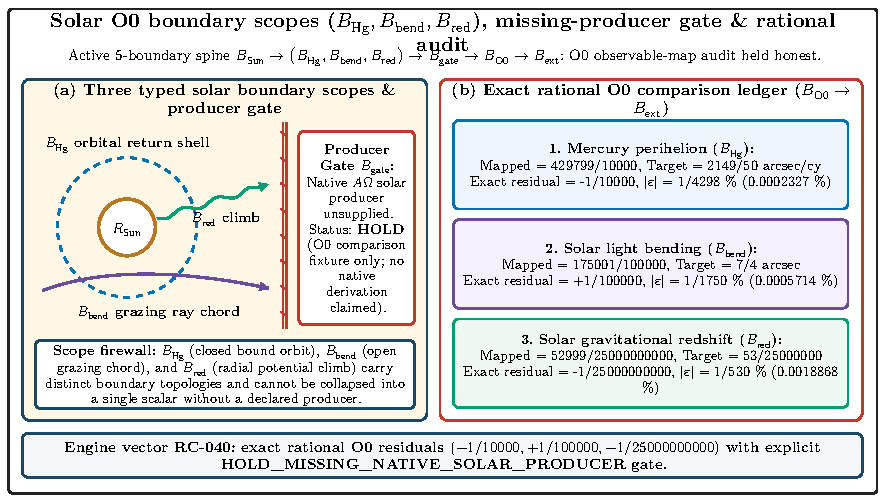
\includegraphics[width=0.92\linewidth,height=0.78\textheight,keepaspectratio]{figures/generated/solar-boundary-scopes-feynman.pdf}
\caption{Typed solar boundary scopes ($B_{\mathrm{Hg}},B_{\mathrm{bend}},B_{\mathrm{red}}$), explicit \texttt{HOLD\_MISSING\_NATIVE\_SOLAR\_PRODUCER} gate, and exact rational O0 comparison ledger (\texttt{RC-040}, \texttt{solar\_o0\_boundary\_dec\_audit.csv}).}
\label{fig:manual-solar-boundary-scopes-feynman}
\end{figure}

\begin{table}[H]
\centering
\caption{Engine-bound exact rational solar O0 observable-map residual and missing-producer gate ledger (\texttt{RC-040}, live from \texttt{solar\_o0\_boundary\_dec\_audit.csv}).}
\label{tab:manual-solar-dec-boundary-audit}
{\scriptsize
\begin{tabular}{>{\raggedright\arraybackslash}p{0.120\linewidth}>{\raggedright\arraybackslash}p{0.120\linewidth}>{\raggedleft\arraybackslash}p{0.128\linewidth}>{\raggedleft\arraybackslash}p{0.096\linewidth}>{\raggedleft\arraybackslash}p{0.112\linewidth}>{\raggedleft\arraybackslash}p{0.064\linewidth}>{\raggedright\arraybackslash}p{0.160\linewidth}}
\toprule
Record & Typed scope & Mapped exact & Target exact & Exact residual & Abs. \% (exact / 7dp) & Producer gate \\
\midrule
\texttt{mercury\_\allowbreak{}perihelion} & \texttt{B\_\allowbreak{}Hg(\allowbreak{}orbital\_\allowbreak{}return\_\allowbreak{}shell)} & 429799/\allowbreak{}10000 & 2149/\allowbreak{}50 & $-$1/\allowbreak{}10000 & 1/4298\par 0.0002327 & \texttt{HOLD\_\allowbreak{}MISSING\_\allowbreak{}NATIVE\_\allowbreak{}SOLAR\_\allowbreak{}PRODUCER} \\
\texttt{solar\_\allowbreak{}light\_\allowbreak{}bending} & \texttt{B\_\allowbreak{}bend(\allowbreak{}grazing\_\allowbreak{}ray\_\allowbreak{}chord)} & 175001/\allowbreak{}100000 & 7/\allowbreak{}4 & 1/\allowbreak{}100000 & 1/1750\par 0.0005714 & \texttt{HOLD\_\allowbreak{}MISSING\_\allowbreak{}NATIVE\_\allowbreak{}SOLAR\_\allowbreak{}PRODUCER} \\
\texttt{solar\_\allowbreak{}redshift} & \texttt{B\_\allowbreak{}red(\allowbreak{}radial\_\allowbreak{}climb\_\allowbreak{}window)} & 52999/\allowbreak{}25000000000 & 53/\allowbreak{}25000000 & $-$1/\allowbreak{}25000000000 & 1/530\par 0.0018868 & \texttt{HOLD\_\allowbreak{}MISSING\_\allowbreak{}NATIVE\_\allowbreak{}SOLAR\_\allowbreak{}PRODUCER} \\
\bottomrule
\end{tabular}
}
\end{table}
